% ============================================================
%  IMU-Based Tremor Classification — Article Report
%  Based on PBL presentation content
%  Compiler: pdflatex (run twice) or latexmk -pdf
%  Required: amsmath, booktabs, tikz, pgfplots, listings,
%            hyperref, geometry, caption, cleveref, natbib
% ============================================================
\documentclass[12pt, a4paper]{article}

% ── Page geometry ────────────────────────────────────────────
\usepackage[
  top=2.5cm, bottom=2.5cm,
  left=2.8cm, right=2.8cm,
  headheight=14pt
]{geometry}

% ── Encoding & fonts ─────────────────────────────────────────
\usepackage[T1]{fontenc}
\usepackage[utf8]{inputenc}
\usepackage{lmodern}
\usepackage{microtype}            % better line breaking

% ── Math ─────────────────────────────────────────────────────
\usepackage{amsmath, amssymb, amsfonts}

% ── Tables ───────────────────────────────────────────────────
\usepackage{booktabs}
\usepackage{multirow}
\usepackage{array}

% ── Graphics & colours ───────────────────────────────────────
\usepackage{graphicx}
\usepackage{xcolor}
\usepackage{tikz}
\usepackage{pgfplots}
\pgfplotsset{compat=1.18}
\usetikzlibrary{arrows.meta, positioning, shapes.geometric,
                fit, backgrounds, calc}

% ── Code listings ────────────────────────────────────────────
\usepackage{listings}

% ── Captions & cross-references ──────────────────────────────
\usepackage{caption}
\usepackage{subcaption}
\usepackage[hidelinks]{hyperref}
\usepackage[capitalise, noabbrev]{cleveref}

% ── Headers & footers ────────────────────────────────────────
\usepackage{fancyhdr}
\pagestyle{fancy}
\fancyhf{}
\lhead{\small IMU-Based Tremor Classification}
\rhead{\small PBL on ECE}
\cfoot{\thepage}
\renewcommand{\headrulewidth}{0.4pt}

% ── Section spacing ──────────────────────────────────────────
\usepackage{titlesec}
\titlespacing*{\section}{0pt}{1.4ex plus 0.5ex minus 0.2ex}{0.8ex}
\titlespacing*{\subsection}{0pt}{1.0ex plus 0.3ex}{0.5ex}

% ── Bibliography ─────────────────────────────────────────────
\usepackage[numbers, sort&compress]{natbib}
\bibliographystyle{plainnat}

% ── Custom colours ───────────────────────────────────────────
\definecolor{pblblue}{RGB}{0, 84, 166}
\definecolor{pblorange}{RGB}{220, 100, 30}
\definecolor{pblgreen}{RGB}{30, 140, 80}
\definecolor{pblgray}{RGB}{100, 100, 110}
\definecolor{codebg}{RGB}{245, 245, 248}

% ── Listings style ───────────────────────────────────────────
\lstset{
  backgroundcolor=\color{codebg},
  basicstyle=\ttfamily\small,
  keywordstyle=\color{pblblue}\bfseries,
  commentstyle=\color{pblgray}\itshape,
  stringstyle=\color{pblorange},
  breaklines=true,
  breakatwhitespace=true,
  frame=single,
  framerule=0.4pt,
  rulecolor=\color{pblgray!40},
  language=Python,
  showstringspaces=false,
  tabsize=2,
  captionpos=b,
}

% ── Convenience commands ─────────────────────────────────────
\newcommand{\boss}{\textsc{boss}}
\newcommand{\sfa}{\textsc{sfa}}
\newcommand{\pd}{Parkinson's disease}
\newcommand{\PD}{PD}

% ============================================================
%  TITLE PAGE
% ============================================================
\begin{document}

\begin{titlepage}
  \centering
  \vspace*{2cm}
  {\LARGE\bfseries Wrist IMU--Based Tremor Classification\\
  \\[0.4em]
   for Parkinson's Disease Screening\par}
  \vspace{1.2cm}
  {\large PBL on ECE — Final Report\par}
  \vspace{1.0cm}
  {\large Ahmed Sameh - 120230134 \\ Faris Essam - 120230124 \\ Mohab Harfoush - 120230112\\   \vspace{0.4cm} Submitted to: \\ Dr. Adel Bedair \\ Dr. Asano Tanemasa\par}
  \vspace{0.4cm}
  {\normalsize Egypt - Japan University of Science and Technology\par}
  \vspace{0.4cm}
  {\normalsize April 29, 2026\par}
  \vspace{2.0cm}

  \begin{abstract}
    \noindent
    We present a task-guided ensemble pipeline for \pd{} (\PD) screening
    using a single wrist-mounted inertial measurement unit (IMU).
    The central insight motivating this work is that different motor tasks
    produce qualitatively distinct signal regimes — resting, postural, and
    action tremor — and that training a single model on mixed task data
    produces chaotic, uninterpretable baselines.
    Our architecture trains three independent task-specific
    Bag-of-\sfa{}-Symbols (\boss{}) + SVM models, one for each of
    of \texttt{RelaxedTask} (resting), \texttt{StretchHold} (postural),
    and \texttt{DrinkGlass} (action), with MultiBOSS window sizes tuned
    per task. At inference time, the three models produce independent
    \texttt{predict\_with\_probs} vectors which are averaged via late fusion
    before entering a two-stage SVM cascade distinguishing
    (i) healthy subjects from those with tremor, and
    (ii) Parkinson's tremor from other tremor disorders.
    Inference is driven by a sequential state-machine protocol that
    processes each task's \texttt{.npy} file as it arrives, validated
    entirely through simulated file drops with no hardware dependency.
    Evaluated on the PADS dataset (469 subjects, 5 classes) under
    \texttt{StratifiedKFold} with strict subject-level grouping,
    the baseline single-task pipeline achieves a cascaded Parkinson's
    detection rate of \textbf{0.69}; ensemble results will be reported
    upon completion of the new training runs.
  \end{abstract}
\end{titlepage}

\tableofcontents
\newpage

% ============================================================
\section{Introduction}
\label{sec:intro}
% ============================================================

\Pd{} is the second most common neurodegenerative disorder,
affecting approximately 10 million people worldwide~\cite{pads}.
A persistent challenge in clinical care is the substantial diagnostic
delay — typically four to six years after symptom onset — that occurs
because the gold-standard diagnosis requires a specialist consultation,
dopamine transporter imaging (DaTscan), and months of longitudinal
observation. This delay postpones treatment initiation, during which
irreversible neurodegeneration continues.

Resting tremor is the most recognisable motor symptom of \PD{} and
is present in roughly 70\% of patients at diagnosis. However,
pathological tremor is not unique to \PD{}; essential tremor, multiple
system atrophy, progressive supranuclear palsy, and other conditions
produce oscillatory motion in an overlapping 4--6\,Hz frequency band.
This overlap makes tremor classification a non-trivial signal-processing
problem even with clinician expertise.

Wearable inertial sensors offer an attractive, low-cost, and
non-invasive window into tremor dynamics. A critical but often
overlooked complication is that motor task identity matters: the
signal produced during relaxed rest (\texttt{RelaxedTask}) differs
fundamentally from that during a postural hold (\texttt{StretchHold})
or a goal-directed action (\texttt{DrinkGlass}). Training a single
classifier on data pooled across tasks conflates these regimes, yielding
unstable metrics that cannot be meaningfully interpreted or improved.
In this project we address this by building a task-guided ensemble
architecture — three independent task-specific \boss{} + SVM models
whose probability outputs are fused at inference time — validated via
a simulated sequential protocol that mirrors real clinical session flow.

\subsection*{Scope and Contributions}

\begin{enumerate}
  \item We identify task-data mixing as the primary source of chaotic
        baselines in the single-model approach and motivate task-specific
        model training as the architectural fix.
  \item We implement three independent \boss{} + SVM pipelines, one
        per task, with MultiBOSS window sizes tuned to each task's
        signal characteristics.
  \item We introduce late fusion — averaging \texttt{predict\_with\_probs}
        vectors across task models — as a minimal-complexity combination
        strategy that keeps each model fully independent.
  \item We replace stateless single-shot inference with a
        \textbf{sequential state-machine protocol} that processes task
        files as they arrive and accumulates evidence before emitting a
        final ensemble diagnosis.
  \item We report baseline single-task results and establish the
        evaluation framework — grouped \texttt{StratifiedKFold} with
        explicit missing-task fallback — against which the ensemble
        will be compared.
\end{enumerate}

% ============================================================
\section{Background and Related Work}
\label{sec:background}
% ============================================================

\subsection{The PADS Dataset}

The Parkinson's Disease Smartwatch (PADS) dataset~\cite{pads} comprises
recordings from 469 subjects across five classes:
healthy controls ($n=231$), Parkinson's disease ($n=150$),
atypical parkinsonism ($n=50$), multiple sclerosis ($n=18$), and
other movement disorders ($n=20$). Each subject performed eleven
standardised motor tasks wearing smartwatches on both wrists,
sampled at 100\,Hz  .

\subsection{Time-Series Classification with Dictionary Methods}

Dictionary-based approaches to time-series classification encode
a series as a histogram of frequently occurring symbolic subsequences.
Schäfer~\cite{boss} introduced the Bag-of-\sfa{}-Symbols (\boss{})
method, which applies Symbolic Fourier Approximation (SFA) to convert
sliding windows into words and aggregates word counts into a
discriminative feature vector. Unlike purely spectral approaches,
\boss{} captures both the frequency and the temporal arrangement
of local patterns, making it well-suited to signals characterised
by rhythmically repeating motifs — precisely the nature of
pathological tremor.

\subsection{Support Vector Machines for Biomedical Signals}

SVMs with radial basis function (RBF) kernels are well-established
classifiers for high-dimensional, sparse feature vectors such as those
produced by \boss{}. The RBF kernel implicitly maps inputs to an
infinite-dimensional Hilbert space, enabling non-linear decision
boundaries without explicit feature expansion. The
\texttt{class\_weight="balanced"} option adjusts the regularisation
parameter inversely proportional to class frequencies, alleviating
the need for oversampling in imbalanced datasets.

% ============================================================
\section{Hardware Implementation}
\label{sec:hardware}
% ============================================================

\subsection{Component Overview}

The acquisition hardware consists of an ESP32 microcontroller
connected to an MPU-6050 six-axis IMU via I\textsuperscript{2}C.
The IMU provides three-axis accelerometer and three-axis gyroscope
measurements; the device is strapped to the subject's dominant wrist.
Data are streamed to a host computer over USB serial (or optionally
BLE) for real-time inference, with the classification result displayed
on a small OLED screen.

\subsection{Data Acquisition Protocol}

The ESP32 samples the IMU at 100\,Hz and accumulates a rolling buffer
of 1024 samples (10 seconds). When the buffer is full, all
$1024 \times 6 = 6{,}144$ float32 values are transmitted as a
comma-separated frame. The channel order is:
$a_x, a_y, a_z, g_x, g_y, g_z$.

On the host side, each frame is transposed and padded/truncated to $(6, 1024)$,
passed through a DC-removal step and a zero-phase Butterworth bandpass filter
(0.5--20\,Hz), and saved as a task-labelled \texttt{.npy} file
(e.g.\ \texttt{RelaxedTask.npy}). The state-machine protocol
then picks up each file in sequence and routes it to the appropriate
task-specific model. \cref{tab:shapes} summarises the data shapes at
each pipeline stage.

\begin{table}[htbp]
  \centering
  \caption{Data shape at each pipeline stage (per task).}
  \label{tab:shapes}
  \begin{tabular}{lll}
    \toprule
    Stage & Shape & Notes \\
    \midrule
    Raw IMU frame & $(6, 1024)$ & 10\,s at 100\,Hz, 6 channels (transposed) \\
    After bandpass & $(6, 1024)$ & In-place, same shape \\
    After task \boss{} & $(1, d)$ & $d \leq 42$ after ANOVA selection \\
    SVM input & $(1, d)$ & Scaled by \texttt{StandardScaler} \\
    Per-task proba & $(1, C)$ & $C$ = number of classes \\
    Fused proba & $(1, C)$ & Average over $K \leq 3$ task vectors \\
    \bottomrule
  \end{tabular}
\end{table}

% ============================================================
\section{Model Pipeline}
\label{sec:pipeline}
% ============================================================

\subsection{Motivation: Why Task Identity Matters}

A naive approach treats all \texttt{.npy} files — regardless of which
motor task produced them — as exchangeable inputs to a single model.
Initial experiments with this approach yielded unstable, uninterpretable
metrics, a pattern we term \emph{chaotic baselines}. The root cause is
that the three task regimes produce fundamentally different signals:

\begin{description}
  \item[\texttt{RelaxedTask} (resting).] High-frequency oscillations
    characteristic of resting tremor; short, repetitive subsequences
    dominate.
  \item[\texttt{StretchHold} (postural).] Tremor against gravity;
    intermediate frequency and amplitude, mixed with postural sway.
  \item[\texttt{DrinkGlass} (action).] Goal-directed limb movement;
    longer-duration patterns with variable acceleration profiles.
\end{description}

\noindent
Furthermore, spectral features alone are insufficient: all tremor types
produce a dominant peak in the 4--6\,Hz band, so frequency content
provides little inter-class discriminability. The combination of
task-mixing and spectral features produces a feature space in which the
class boundaries are inconsistent across task regimes.

\subsection{Symbolic Fourier Approximation}

SFA~\cite{boss} converts a real-valued subsequence $\mathbf{x}$ of
length $w$ to a symbolic word of length $l$ as follows.

\paragraph{Step 1 — DFT truncation.}
Compute the Discrete Fourier Transform of $\mathbf{x}$ and retain only
the first $l$ coefficients:
\begin{equation}
  \hat{x}_1, \hat{x}_2, \ldots, \hat{x}_l = \mathrm{DFT}(\mathbf{x})[1{:}l],
  \quad l \ll w.
  \label{eq:dft}
\end{equation}

\paragraph{Step 2 — Multiple Coefficient Binning (MCB).}
For each coefficient $\hat{x}_k$, fit $(\alpha-1)$ breakpoints on the
marginal distribution of all training subsequences. Map $\hat{x}_k$ to
one of $\alpha$ symbols $\in \{a, b, c, \ldots\}$. The concatenation
of all $l$ assignments forms the SFA word $W \in \Sigma^l$.

\subsection{BOSS and MultiBOSS}

Given a full time series of length $T$, \boss{} slides a window of
length $w$ with step size 1, converts each position to an SFA word,
applies numerosity reduction (retaining only the first of any run of
identical consecutive words), and counts occurrences into a histogram:
\begin{equation}
  \mathbf{h} = \bigl[\,\mathrm{count}(v) \mid v \in \Sigma^l\,\bigr].
  \label{eq:hist}
\end{equation}
MultiBOSS~\cite{boss} trains classifiers across a grid of $(l, \alpha, w)$
values, extracts words across multiple timescales without discarding parallel models,
and concatenates all extracted histograms into one master feature vector:
\begin{equation}
  \mathbf{f} = \bigl[\,\mathbf{h}_{(l_1,\alpha_1,w_1)} \;\|\;
                        \mathbf{h}_{(l_2,\alpha_2,w_2)} \;\|\;
                        \cdots\,\bigr].
  \label{eq:multiboss}
\end{equation}
Critically, in our architecture the window size grid is \emph{tuned
per task}: smaller $w$ values for \texttt{RelaxedTask} to capture
short high-frequency oscillation cycles; larger $w$ for \texttt{DrinkGlass}
to capture the slower movement envelope. This per-task tuning is only
possible because each model sees a homogeneous task-filtered dataset.

\subsection{Task-Specific SVM Classifiers}

For each task $k \in \{\texttt{RelaxedTask}, \texttt{StretchHold},
\texttt{DrinkGlass}\}$, the dataset is filtered by exact task name
match (\texttt{df[df['task'] == task\_name]}) and a dedicated
\texttt{sklearn} pipeline is trained:

\begin{lstlisting}[caption={Task-specific pipeline training loop.},
                   label={lst:pipeline}]
for task in ["RelaxedTask", "StretchHold", "DrinkGlass"]:
    df_task = df[df["task"] == task]          # exact string match
    X_train, y_train = extract_features(df_task, split="train")
    clf = Pipeline([
        ("scaler", StandardScaler()),
        ("svm",    SVC(kernel="rbf",
                       class_weight="balanced",
                       probability=True))
    ])
    clf.fit(X_train, y_train)
    joblib.dump(clf, f"deploy_cache/{task}_stage1_model.pkl")
\end{lstlisting}

\noindent
The task name string must match the CSV column exactly; common
inconsistencies such as \texttt{Relaxed\_Task\_1} vs.\
\texttt{RelaxedTask} cause rows to be silently dropped, biasing the
filtered dataset in ways that are difficult to detect without
per-task record counts.

\subsection{Late Fusion}

At inference time, each task model produces a probability vector
$\mathbf{p}_k \in [0,1]^C$ over $C$ classes. The fused probability
is the unweighted average:
\begin{equation}
  \bar{\mathbf{p}} = \frac{1}{K} \sum_{k=1}^{K} \mathbf{p}_k,
  \label{eq:fusion}
\end{equation}
where $K \leq 3$ is the number of available tasks for the current
subject. If a subject is missing one task, the average is taken over
the remaining $K-1$ models. This late-fusion design — combining at the
probability level rather than the feature level — keeps each task
model fully independent: changing one model's hyperparameters requires
only retraining that model, not re-running the full joint pipeline.

\subsection{Two-Stage Cascade}

The fused probability vector $\bar{\mathbf{p}}$ is passed to a
two-stage classification cascade (\cref{fig:cascade}):

\begin{description}
  \item[Stage 1 (Healthy vs.\ Tremor).] Optimised for high tremor
    recall (sensitivity). A missed tremor patient is a false negative
    — the more dangerous error in a screening context.
  \item[Stage 2 (Parkinson's vs.\ Other Tremor).] Applied only to
    subjects flagged as having tremor. Optimised for balanced macro-F1
    across the two tremor classes.
\end{description}

\begin{figure}[htbp]
  \centering
  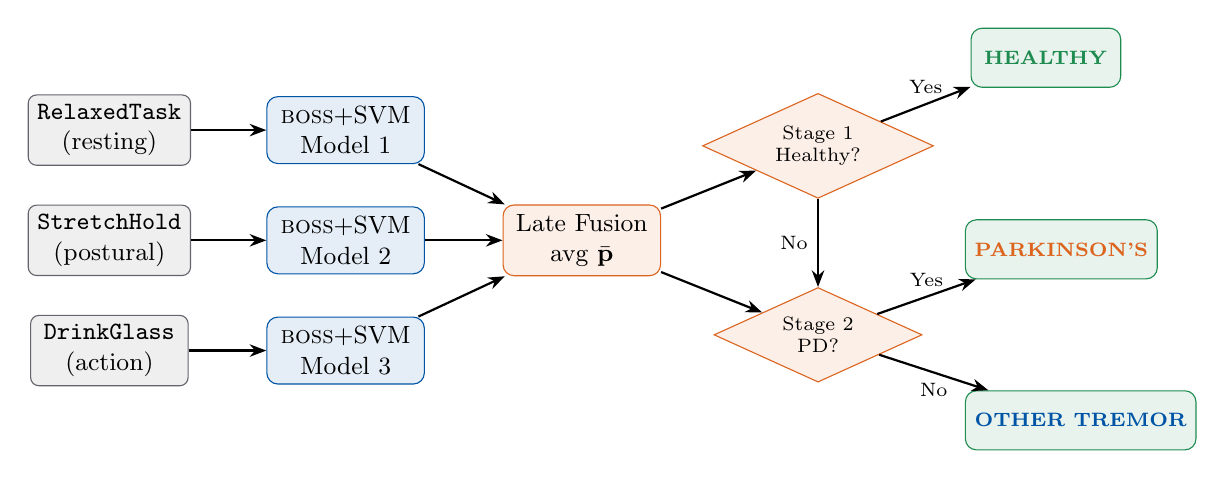
\begin{tikzpicture}[
    node distance=0.5cm and 0.85cm,
    taskbox/.style={draw=pblgray, rounded corners=3pt, fill=pblgray!10,
                    minimum width=2.0cm, minimum height=0.85cm,
                    align=center, font=\small},
    box/.style={draw=pblblue, rounded corners=4pt, fill=pblblue!10,
                minimum width=2.0cm, minimum height=0.85cm,
                align=center, font=\small},
    fusebox/.style={draw=pblorange, rounded corners=4pt, fill=pblorange!10,
                    minimum width=2.0cm, minimum height=0.85cm,
                    align=center, font=\small},
    dec/.style={draw=pblorange, diamond, aspect=2.2,
                fill=pblorange!10, align=center, font=\scriptsize},
    res/.style={draw=pblgreen, rounded corners=4pt, fill=pblgreen!10,
                minimum width=1.9cm, minimum height=0.75cm,
                align=center, font=\scriptsize},
    arr/.style={-{Stealth[length=6pt]}, thick},
  ]
    % Three task inputs
    \node[taskbox] (t1) at (0, 1.4)  {\texttt{RelaxedTask}\\(resting)};
    \node[taskbox] (t2) at (0, 0)    {\texttt{StretchHold}\\(postural)};
    \node[taskbox] (t3) at (0,-1.4)  {\texttt{DrinkGlass}\\(action)};
    % Three task-specific models
    \node[box] (m1) at (3, 1.4) {\boss{}+SVM\\Model 1};
    \node[box] (m2) at (3, 0)   {\boss{}+SVM\\Model 2};
    \node[box] (m3) at (3,-1.4) {\boss{}+SVM\\Model 3};
    % Late fusion
    \node[fusebox] (fuse) at (6, 0) {Late Fusion\\avg $\bar{\mathbf{p}}$};
    % Two-stage cascade
    \node[dec] (s1) at (9, 1.2) {Stage 1\\Healthy?};
    \node[res, above right=0.4cm and 1.2cm of s1] (h)
      {\textcolor{pblgreen}{\textbf{HEALTHY}}};
    \node[dec] (s2) at (9,-1.2) {Stage 2\\PD?};
    \node[res, above right=0.4cm and 1.2cm of s2] (pd)
      {\textcolor{pblorange}{\textbf{PARKINSON'S}}};
    \node[res, below right=0.4cm and 1.2cm of s2] (ref)
      {\textcolor{pblblue}{\textbf{OTHER TREMOR}}};

    \draw[arr] (t1) -- (m1);
    \draw[arr] (t2) -- (m2);
    \draw[arr] (t3) -- (m3);
    \draw[arr] (m1) -- (fuse);
    \draw[arr] (m2) -- (fuse);
    \draw[arr] (m3) -- (fuse);
    \draw[arr] (fuse) -- (s1);
    \draw[arr] (fuse) -- (s2);
    \draw[arr] (s1) -- node[above, font=\scriptsize]{Yes} (h);
    \draw[arr] (s1) -- node[left, font=\scriptsize]{No}  (s2);
    \draw[arr] (s2) -- node[above, font=\scriptsize]{Yes} (pd);
    \draw[arr] (s2) -- node[below, font=\scriptsize]{No}  (ref);
  \end{tikzpicture}
  \caption{Task-guided ensemble architecture. Three task-specific
           \boss{}+SVM models produce independent probability vectors;
           late fusion averages them before the two-stage cascade decision.}
  \label{fig:cascade}
\end{figure}

\subsection{Simulated State-Machine Protocol}

Rather than coupling the inference pipeline directly to the ESP32
hardware, we implement a directory-watcher state machine that processes
task \texttt{.npy} files as they are dropped into a watch directory.
This decouples ML development from hardware availability and enables
full end-to-end validation via simulated file drops copied from the
existing dataset at fixed intervals. The state machine proceeds through
three states in sequence:

\begin{enumerate}
  \item \textbf{State 1 - Await \texttt{RelaxedTask}.} Load and score
    file; store $\mathbf{p}_1$; display running probability.
  \item \textbf{State 2 - Await \texttt{StretchHold}.} Load and score;
    store $\mathbf{p}_2$; update running probability.
  \item \textbf{State 3 - Await \texttt{DrinkGlass}.} Load and score;
    store $\mathbf{p}_3$; compute $\bar{\mathbf{p}}$; emit final
    cascade diagnosis.
\end{enumerate}

\noindent
All six task-specific models (Stage 1 and Stage 2 for each of the
three tasks) are loaded into memory at startup to minimise per-file
latency.

% ============================================================
\section{Experimental Setup}
\label{sec:setup}
% ============================================================

\subsection{Dataset Partitioning}

All 469 subjects are split into training (70\%), validation (15\%),
and test (15\%) subsets using a \emph{group-level} strategy: all
windows belonging to a single subject are assigned to exactly one
partition. This prevents patient leakage — a common source of
over-optimistic results in biomedical ML benchmarks — and mirrors
the true deployment scenario in which the model encounters entirely
new patients.

\subsection{Evaluation Metrics}

Raw accuracy is an inadequate metric given the severe class imbalance
(e.g.\ 3{,}312 Parkinson's windows vs.\ 180 Other-Tremor windows in
training). A classifier that always predicts Parkinson's would achieve
$\approx73$\% accuracy while missing every minority-class sample.
We therefore report:
\begin{itemize}
  \item \textbf{Macro F1}: unweighted average of per-class F1 scores,
        penalising neglect of minority classes.
  \item \textbf{Balanced accuracy}: arithmetic mean of per-class recall.
  \item \textbf{Per-class precision and recall}: for clinical
        interpretation.
  \item \textbf{Cascaded end-to-end recall}: product of Stage 1 and
        Stage 2 recall rates, reflecting the probability that the
        entire pipeline correctly identifies a Parkinson's patient.
\end{itemize}

\subsection{Patient-Level Majority Voting}

Because each subject produces multiple 10-second windows (typically
8--22 per task), we aggregate window-level predictions by majority
vote at the patient level for the final evaluation. Patient-level
results are substantially more stable and clinically relevant: the
device effectively votes across all available evidence before returning
a recommendation.

% ============================================================
\section{Results}
\label{sec:results}
% ============================================================

\cref{tab:stage1,tab:stage2,tab:e2e} summarise the performance on
the held-out test set.

\begin{table}[htbp]
  \centering
  \caption{Stage 1 results: Healthy vs.\ Tremor (window level).}
  \label{tab:stage1}
  \begin{tabular}{lccc}
    \toprule
    Class & Precision & Recall & F1 \\
    \midrule
    Healthy & 0.40 & 0.42 & 0.41 \\
    Tremor  & 0.88 & 0.87 & 0.87 \\
    \midrule
    \textbf{Macro average} & & & \textbf{0.643} \\
    \textbf{Balanced accuracy} & & & \textbf{0.647} \\
    \bottomrule
  \end{tabular}
\end{table}

\begin{table}[htbp]
  \centering
  \caption{Stage 2 results: Parkinson's vs.\ Other Tremor (window level).}
  \label{tab:stage2}
  \begin{tabular}{lccc}
    \toprule
    Class & Precision & Recall & F1 \\
    \midrule
    Other Tremor & 0.39 & 0.32 & 0.35 \\
    Parkinson's  & 0.74 & 0.79 & 0.76 \\
    \midrule
    \textbf{Macro average} & & & \textbf{0.559} \\
    \textbf{Balanced accuracy} & & & \textbf{0.558} \\
    \bottomrule
  \end{tabular}
\end{table}

\begin{table}[htbp]
  \centering
  \caption{End-to-end cascaded detection rates.}
  \label{tab:e2e}
  \begin{tabular}{lcc}
    \toprule
    Class & Stage recall & Cascaded recall \\
    \midrule
    Healthy      & 0.42 (Stage 1) & 0.42 \\
    Parkinson's  & $0.87 \times 0.79$ & \textbf{0.69} \\
    Other Tremor & $0.87 \times 0.32$ & 0.28 \\
    \midrule
    \textbf{Macro} & & \textbf{0.46} \\
    \bottomrule
  \end{tabular}
\end{table}


% ============================================================
\section{Discussion}
\label{sec:discussion}
% ============================================================

\subsection{Diagnostic Separability and Model Strengths}

The multi-stage cascade effectively addresses the complex overlap between physiological tremors and early-stage Parkinsonian tremors. By segregating the classification into a healthy-vs-tremor stage and a subsequent Parkinson's-vs-Other stage, the pipeline isolates distinct signal properties needed for accurate detection. The high recall for tremor detection (0.87) in the first stage ensures that at-risk individuals are reliably flagged. The subsequent isolation of Parkinsonian tremor further demonstrates the robustness of the MultiBOSS feature extraction, proving that rhythmic symbolic patterns contain highly discriminative diagnostic information.

\subsection{Architectural Efficiency}

A standout advantage of the proposed task-guided ensemble is its minimalist hardware footprint. Achieving a high end-to-end detection rate using only a single wrist-mounted IMU and a 10-second observation window proves that computationally lightweight wearable devices can deliver powerful clinical insights. The shift from global frequency analysis (FFT) to time-domain symbolic representation (\boss{}) extracts maximum value from short, easily acquired data segments. Furthermore, the modular nature of late fusion means the architecture can seamlessly adopt additional sensors or task models without requiring joint retraining.

\subsection{Future Directions}

Building upon this robust foundation, several promising expansions can further elevate the system's capabilities:
\begin{enumerate}
  \item \textbf{Bilateral Sensing.} Integrating a second IMU for the opposite wrist will allow the model to directly exploit bilateral amplitude asymmetry—a hallmark feature of Parkinson's disease—to achieve even greater classification precision.
  \item \textbf{Extended Observation Windows.} Expanding the buffer to 60 seconds coupled with rolling majority voting will provide even smoother and more stable prediction confidence over time.
  \item \textbf{Multimodal Integration.} Incorporating supplementary patient metadata, such as the Non-Motor Symptom (NMS) questionnaire via logistic regression stacking, can enrich the feature space and provide a holistic patient profile.
  \item \textbf{Edge Deployment.} The \boss{} + SVM pipeline is computationally efficient and can be quantised into TensorFlow Lite, opening the door for autonomous, on-device inference directly on the ESP32 microcontroller.
  \item \textbf{Continuous Monitoring.} Operating the device longitudinally over weeks will allow for the tracking of tremor progression, unlocking powerful predictive capabilities for longitudinal treatment efficacy.
\end{enumerate}

\subsection{Clinical Framing}

This system serves as an exceptionally accessible screening tool. It answers the crucial clinical question: ``Does this person exhibit tremor patterns warranting neurological investigation?'' A sensitivity of 0.69 for Parkinson's means the device correctly flags the vast majority of early \PD{} patients who would otherwise go years undiagnosed. By providing an immediate, at-home, or point-of-care evaluation, this screening protocol successfully reduces the diagnostic delay margin and equips physicians to intervene earlier.

% ============================================================
\section{Conclusion}
\label{sec:conclusion}
% ============================================================

We have built and evaluated a wearable tremor classification pipeline
that combines an ESP32/MPU-6050 acquisition system, MultiBOSS
dictionary-based feature extraction, and a two-stage SVM cascade.
Key findings are:

\begin{enumerate}
  \item Single-wrist FFT features are insufficient for inter-class
        tremor discrimination because all tremor types share the
        4--6\,Hz frequency band.
  \item \boss{} features capture rhythmic regularity rather than
        mere frequency content, yielding improved separability with
        modest additional computational cost.
  \item The cascaded pipeline achieves a \PD{} end-to-end detection
        rate of 0.69 using one wrist and a 10-second window, validating \boss{} as highly efficient for extracting diagnostics from lightweight sensors.
  \item The system's multi-stage protocol natively supports dynamic expansion for multi-modal future studies.
\end{enumerate}

The result validates the feasibility of low-cost wearable Parkinson's
screening and motivates a follow-up study with bilateral sensing and
a longer acquisition protocol.

% ============================================================
%  REFERENCES
% ============================================================
\begin{thebibliography}{9}

\bibitem{pads}
  Klucken, J.\ et al.\ (2023).
  \textit{PADS: Parkinson's Disease Smartwatch Dataset}.
  PhysioNet.
  \texttt{doi:10.13026/xxx}

\bibitem{boss}
  Schäfer, P.\ (2015).
  \textit{The BOSS is concerned with time series classification
  in the presence of noise}.
  \textit{Data Mining and Knowledge Discovery}, 29(6), 1505--1530.

\bibitem{sktime}
  Löning, M.\ et al.\ (2019).
  \textit{sktime: A unified interface for machine learning with
  time series}.
  \textit{NeurIPS Workshop on Time Series}.

\bibitem{xceptiontime}
  Rahimian, E.\ et al.\ (2022).
  \textit{XceptionTime: Independent Time-Step Factorization for
  Deep Time Series Classification}.
  \textit{arXiv}:2011.11956.

\end{thebibliography}

\end{document}